\documentclass[11pt,class=article,float=false,crop=false]{standalone}
%\documentclass[11pt]{article}
\usepackage{Part3_packages}

\begin{document}

\section{Détection des collisions}
La phase de détection vise à tester pour chaque paire d'objets s'ils entrent en collision ou non. Nous verrons dans cette partie comment déterminer de manière robuste si la collision à lieu, puis nous nous intéresserons aux méthodes utilisées pour accélérer cette phase de détection en utilisant des méthodes de hiérarchisation de l'espace et de volumes englobants. 

Les techniques utilisées sont principalement inspirées de \citecol{ericson2004real} qui propose un tour d'horizon complet du domaine de la détection de collisions en temps réel.

\subsection{Définition du problème}
La détection de collision est la première étape de l'algorithme de collisions des dislocations qui s'effectue après la phase d'intégration (\textbf{Déplacement} sur la figure \ref{fig:deroulement_simulation}). Le réseau de dislocations est représenté par un maillage composé de noeuds connectés par les segments de dislocations, comme le montre la figure \ref{fig:collision-detection-probleme}. On suppose que les noeuds se déplacent à vitesse constante dans un espace à 3 dimensions pendant un pas de temps $dt$. La position du nœud $i$ est notée $p_i$, et sa vitesse $v_i$.

\begin{figure}[H]
	\centering
	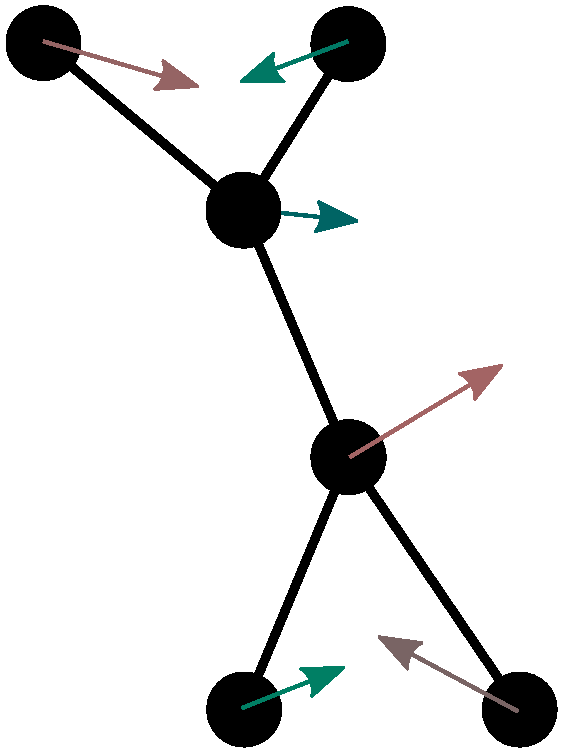
\includegraphics[height=0.2\textheight]{img/collision-detection-probleme}
	\caption{Le réseau de dislocations décoré des vitesses nodale.}
	\label{fig:collision-detection-probleme}
\end{figure}

Le problème à résoudre consiste à détecter quels objets (nœuds ou segments) entrent en contact au cours d'un pas de temps, et à déterminer le temps où le contact à lieu. Deux objets entrent en collision lorsque leur distance de séparation passe sous un certain seuil $\epsilon$\footnote{$\epsilon$ est en fait une autre notation pour $r_{col}$}. La formule \ref{eq:collision} formalise la condition de collision entre deux objets $o_1$ et $o_2$ au cours d'un pas de temps $dt$:

\begin{equation}
\operatorname{collision}(o_1,o_2) \equiv \exists t \in [0,dt] ,  \operatorname{dist}(o_1,o_2) < \epsilon	
\label{eq:collision}
\end{equation}

\paragraph{Note:}
Afin de s'abstraire de la méthode d'intégration utilisée dans la simulation, les vitesses nodales peuvent être calculées à partir des positions initiales et finales pour le pas de temps considéré : 
\begin{equation}
	v_i =  \frac{ p_i(t+dt) - p_i(t) }{dt}
\end{equation}
Cela permet de considérer la vitesse nodale constante malgré que la méthode d'intégration ne soit pas une méthode explicite.



\subsection{Primitives de détection}
\label{sec:primitives_collision}

Les primitives de détection de collision sont des fonctions qui permettent de déterminer si deux objets entrent en collision au cours du pas de temps. On appelle ces primitives pour chaque couple d'objets. Afin de gérer tous les cas qui se présentent à nous, plusieurs primitives doivent être implémentées:
\begin{itemize}
	\item Point/Point;
	\item Point/Segment;
	\item Segment/Segment.
\end{itemize} 

Séparer les primitives permet de gérer les cas particuliers plus facilement : par exemple une collision qui interviendrait au bout d'un segment pourra être considéré comme une collision Point / Segment. Cela permet d'augmenter à la fois la robustesse de la détection, mais aussi la régularité du calcul en évitant les cas particuliers, ce qui permet un meilleure performance.

Lorsque deux points se déplacent dans l'espace, il est très peu probable qu'une collision exacte se produise entre ces 2 points. Pourtant, si ces points s’approchent suffisamment l'un de l'autre, nous voudrions qu'une collision soit détectée. Les primitives présentées ici effectuent des calculs de collision à $\epsilon$ près afin d'éviter les problèmes d'instabilités numériques qui pourraient intervenir, ainsi que pour s'approcher mieux de la réalité physique des dislocations. 

Les primitives suivantes décrivent la manière de calculer la distance entre les objets, et déterminent le choix du temps de collision parmi tous les $t$ qui vérifient la condition $\operatorname{collision}(o1,o2)$ (Équation \ref{eq:collision}). 

\subsubsection{Point/Point}
\label{sec:detection-pointpoint}

La primitive la plus simple détecte la collision entre 2 nœuds du réseau de dislocation. Les nœuds sont représentés par des sphères de rayon $\epsilon$ ayant pour positions initiales $p_1$ et $p_2$, et se déplaçant à vitesse constante $v_1$ et $v_2$, comme l'illustre la figure \ref{fig:collision-primitive-pointpoint}.

\begin{figure}[H]
	\centering
	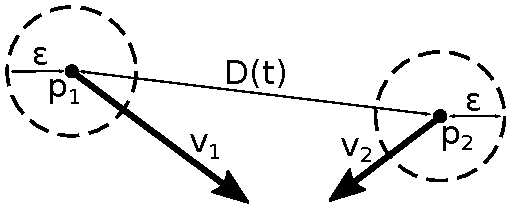
\includegraphics[width=0.5\textwidth]{img/collision-primitive-pointpoint}
	\caption{Distance entre deux nœuds du réseau de dislocations.}
	\label{fig:collision-primitive-pointpoint}
\end{figure}

La distance entre les deux points au cours du temps se calcule de la manière suivante: 

\begin{align}
	D(n_1,n_2) & = \|(p_2+t*v_2)-(p_1+t*v_1)\| \\
	D^2(t)       & = at^2 + bt + c 
\end{align}
avec
\begin{align}
	a & = \|v_2-v_1\|^2 \\
	b & = 2(v_2-v_1 \cdot p_2-p_1) \\
	c & = \|p_2-p_1\|^2
\end{align}

Comme $D^2 > 0$, le polynôme de degré 2 est concave, le minimum de la fonction est atteint en $t_{min} = \frac{-b}{2a}$. Si $t_{min}$ n'est pas dans $[0,dt]$, alors on le ramène dans l'intervalle \footnote{l'opération peut être délicate si $a=0$ : la distance est constante, et $t_{min}=0$}, comme le montre la figure \ref{fig:collision-primitive-pointpoint-polynome}.

\begin{figure}[H]
	\centering
	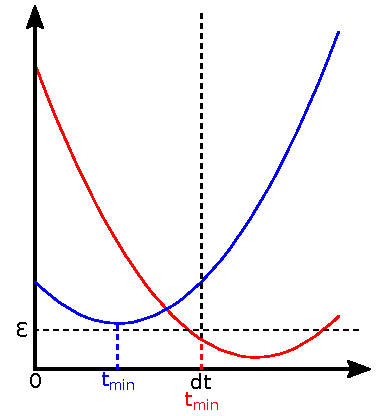
\includegraphics[height=0.3\textheight]{img/collision-primitive-pointpoint-polynome}
	\caption{Distance entre deux nœuds du réseau de dislocations.}
	\label{fig:collision-primitive-pointpoint-polynome}
\end{figure}

Une collision à lieu si la distance est inférieure à $\epsilon$, et le temps de la collision est $t_{min}$ :

\begin{equation}
	\operatorname{collision}(n_1,n_2) \equiv D^2(t_{min}) < \epsilon
\end{equation}

\subsubsection{Point/Segment}

La seconde primitive présentée détecte la collision entre un nœud et un segment. Le nœud est représenté par une sphère de rayon $\epsilon$, et le segment par un cylindre de rayon $\epsilon$. Le segment $s = [n_1,n_2]$ et le nœud $n_3$ ont pour positions et vitesses respectives $p_i$ et $v_i$, comme l'illustre la figure \ref{fig:collision-primitive-pointseg}.

\begin{figure}[H]
	\centering
	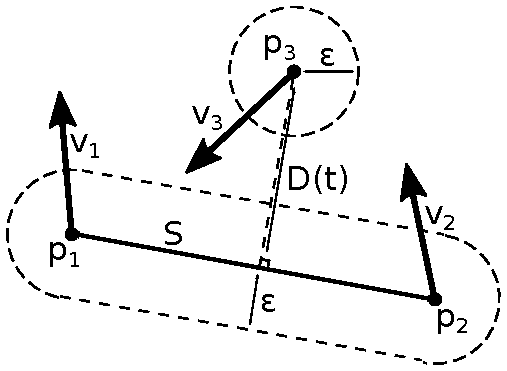
\includegraphics[width=0.5\textwidth]{img/collision-primitive-pointseg}
	\caption{Distance entre un nœud et un segment du réseau de dislocations.}
	\label{fig:collision-primitive-pointseg}
\end{figure}

La distance entre la droite $(s)$ et le point $n_3$ se calcule de la manière suivante: 

\begin{align}
	D(s,n_3) & = \frac{\|\vect{12}(t) \wedge \vect{13}(t)\|}
	{\|\vect{12}(t)\|} \\
	& = \frac{\|(\vect{p_{12}} + t\vect{v_{12}}) \wedge (\vect{p_{13}} + t\vect{v_{13}})\|}
	{\|\vect{12}(t)\|} \\
	& = \frac{\|\vect{a}t^2 + \vect{b}t + \vect{c}\|}
	{\|\vect{12}(t)\|}
\end{align}
avec 
\begin{align}
	\vect{a} &= \vect{v_{12}} \wedge \vect{v_{13}}\\
	\vect{b} &= \vect{v_{12}} \wedge \vect{p_{13}}+ \vect{p_{12}} \wedge \vect{v_{13}}\\
	\vect{c} &= \vect{p_{12}} \wedge \vect{p_{13}}
\end{align}

En passant la distance au carré, on obtient:

\begin{align}
	D^2(s,n_3) & = \frac{\|\vect{a}t^2 + \vect{b}t + \vect{c}\|^2}
	{\|\vect{12}(t)\|^2} \\
	& =  \frac{at^4 + bt^3 + ct^2 + dt + e}
	{\|\vect{12}(t)\|^2} 
\end{align}

avec 

\begin{align}
	a &= \|\vect{a}\|^2\\
	b &= 2(\vect{a} \cdot \vect{b})\\
	c &= \|\vect{b}\|^2 + 2(\vect{a} \cdot \vect{c})\\
	d &= 2(\vect{b} \cdot \vect{c})\\
	e &= \|\vect{c}\|^2
\end{align}

Comme pour la collision point / point, il s'agit maintenant de minimiser la distance entre le segment et le point, et de comparer cette distance minimale à $\epsilon$. Cependant, la fonction distance dans ce cas est difficile à minimiser analytiquement car il n'existe pas de formule simple pour calculer les racines d'un polynôme de degré supérieur à 4. Deux possibilité s'offrent à nous: 

\begin{itemize}
	\item Minimiser numériquement la distance (Dichotomie, Méthode de Newton, ...);
	\item Approximer la distance par une fonction qu'il est possible de minimiser analytiquement. 
\end{itemize}

La méthode choisie consiste à approximer la distance $||\vect{12}(t)||$ par une constante. Cette approximation est justifiée car si $||\vect{12}(t)||$ diminue trop, la collision sera détectée comme une collision entre les points $n_1$ et $n_2$. Le calcul de la distance devient:
\begin{equation}
D^2(t) = \frac{\|\vect{12}(t) \wedge \vect{13}(t)\|^2}
{\|\vect{12}(t)\|^2} \approx \frac{P(t)}
{C^2}
\label{eq:collision-pointseg-approx}
\end{equation}
avec $P$ un polynôme de degré 4.

Minimiser $D^2$ revient à minimiser le polynôme $P$ : nous cherchons les racines de $P^\prime$ pour lesquelles $P^{\prime \prime}$ est positif. $P > 0$, donc il possède au plus deux minimas locaux, comme le montre la figure \ref{fig:collision-primitive-pointseg-polynome}.

\begin{figure}[H]
	\centering
	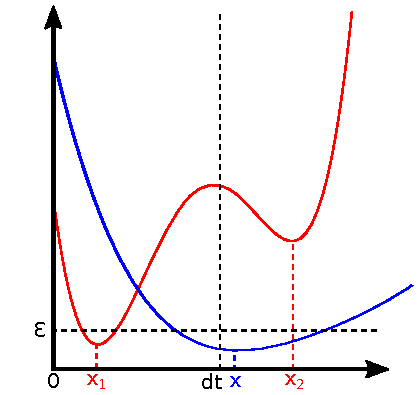
\includegraphics[height=0.3\textheight]{img/collision-primitive-pointseg-polynome}
	\caption{Minimisation de la distance entre un nœud et un segment.}
	\label{fig:collision-primitive-pointseg-polynome}
\end{figure}

Pour les minimas $x_i$ trouvés, il faut tester si $D(x_i) < \epsilon$, mais aussi si le point entre en collision avec la droite à l'intérieur du segment. Le calcul de distance pour la comparaison avec $\epsilon$ doit être effectué à partir des positions des points, et non de l'expression approximée (\ref{eq:collision-pointseg-approx}). Le test d'inclusion au segment peut se faire en vérifiant que les produits scalaires $<\vect{12},\vect{13}>$ et $<\vect{12},\vect{23}>$ sont de signe différents.

Le cas ou la collision survient au bout du segment est déjà géré lors des collisions point / point. Cela permet d'éviter des instabilités numériques lors du calcul de la distance.

\subsubsection{Segment/Segment}

Pour la détection de la collision entre deux segments, les segments sont représentés par des cylindres de rayon $\epsilon$. Les segments $s_1 = [n_1,n_2]$ et $s_2 = [n_3,n_4]$ ont pour positions et vitesses respectives $p_i$ et $v_i$, comme l'illustre la figure \ref{fig:collision-primitive-segseg}

\begin{figure}[H]
	\centering
	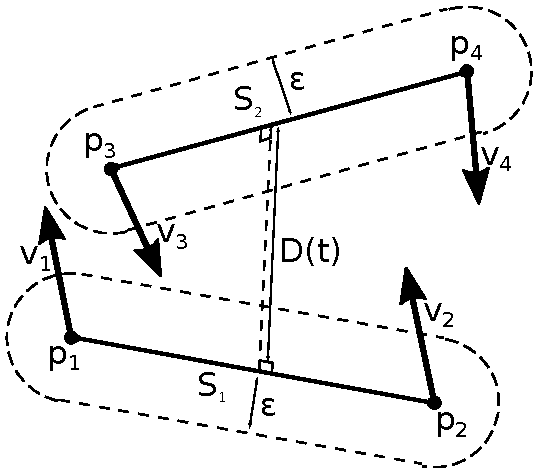
\includegraphics[width=0.5\textwidth]{img/collision-primitive-segseg}
	\caption{Distance entre deux segments du réseau de dislocations.}
	\label{fig:collision-primitive-segseg}
\end{figure}

A ce point, il est important de comprendre que les cas particuliers sont déjà gérés par les primitives précédentes. Par exemple, le cas où les segments sont parallèles est déjà géré par la primitive de détection de collision point / segment, et le cas où l'un des segments serait de longueur nulle est pris en compte par le cas point / point. Il ne nous reste plus qu'a gérer la collision entre segments dans le cas général. 

La distance se calcule de la manière suivante:

\begin{align}
	D(s_1,s_2) & =\frac{ \vect{13}(t) \cdot (\vect{12}(t) \wedge \vect{34}(t))}
	{\|\vect{12}(t) \wedge \vect{34}(t)\|} \\
	& = \frac{det(\vect{13}(t), \vect{12}(t), \vect{34}(t))}
	{\|\vect{12} \wedge \vect{34}\|} 
\end{align}

Comme les primitives précédentes couvrent les cas où $\|\vec{12} \wedge \vec{34}\| = 0$, nous n'avons plus qu'a trouver les racines du déterminant:

\begin{align}
	P(t) &= \operatorname{det}(\vect{13}(t), \vect{12}(t), \vect{34}(t)) \\
	&= \operatorname{det}(\vect{p_{13}}+t~\vect{v_{13}},~ \vect{p_{12}}+t~\vect{v_{12}},~\vect{p_{34}}+t~\vect{v_{34}}))
\end{align}

Par linéarité du déterminant:

\begin{align}
	P(t) =& a\cdot t^3 + b\cdot t^2 + c\cdot t + d \\
	& a = \operatorname{det}(\vect{v_{13}},\vect{v_{12}},\vect{v_{34}})\\
	& b = \operatorname{det}(\vect{p_{13}},\vect{v_{12}},\vect{v_{34}}) 
	+ \operatorname{det}(\vect{v_{13}},\vect{p_{12}},\vect{v_{34}}) 
	+ \operatorname{det}(\vect{v_{13}},\vect{v_{12}},\vect{p_{34}})\\
	& c = \operatorname{det}(\vect{v_{13}},\vect{p_{12}},\vect{p_{34}}) 
	+ \operatorname{det}(\vect{p_{13}},\vect{v_{12}},\vect{p_{34}}) 
	+ \operatorname{det}(\vect{p_{13}},\vect{p_{12}},\vect{v_{34}})\\
	& d = \operatorname{det}(\vect{p_{13}},\vect{p_{12}},\vect{p_{34}})
\end{align}

Contrairement aux expressions précédentes, cette distance est algébrique. Ici nous souhaitons trouver les minimas de $|D|$ qui sont les racines de D mais aussi certains des ses extrema locaux. On résout donc 2 équations: 
\begin{align}
	P(t) &= 0 \\
	P^\prime (t) &= 0 \text{ et } P^{\prime\prime} (t) \text{ de même signe que } P(t) 
\end{align}

Pour chacun de ces minimas, il faut alors tester si $D < \epsilon$, et si le point de collision est bien à l'intérieur des segments. Le temps retenu pour la collision, est la première de ces valeurs.

\subsection{Algorithme de détection}
L'algorithme de détection est chargé d'exécuter les primitives de collisions pour chaque paire d'objets, et de construire une liste des collisions détectées. 

L'algorithme naïf où chaque paire d'objets est testée possède une complexité quadratique. Il peut être utilisé comme algorithme de référence, mais sa complexité est trop importante pour qu'il soit utilisé sur des données massives. Des solutions basées sur la localité spatiale permettent de réduire la complexité de l'algorithme, notamment en triant spatialement les objets et en hiérarchisant l'espace. En effet, certains objets sont souvent trop éloignés les uns des autres pour qu'une collision soit possible.

Dans la littérature, plusieurs solutions existent pour découper l'espace afin de réduire la complexité du calcul. On peut par exemple citer des méthodes utilisant les \textit{bounding volumes}, la hiérarchisation par \textit{BSP-Tree}, etc\dots \citecol{ericson2004real}. Les solutions envisagées ici consistent en un découpage de l'espace en grille régulière, et en l'utilisation de sphères englobantes comme \textit{bounding volumes}.

\subsubsection{Découpage en grille uniforme}
L'espace en 3 dimensions est découpé selon un grille uniforme de manière à ce que les objets présents dans chaque boite ne puisse entrer en collision qu'avec les objets des boites voisines. Pour chaque objet, au lieu de tester la collision avec tous les autres objets du domaine, il suffit de tester la collision avec les objets contenus dans les boites voisines.

Afin de séparer les objets qui n'entrent pas en collision, les boites doivent vérifier la condition suivante:

\begin{equation}
\frac{l_{max}}{2} + v_{max}~dt + \epsilon < \frac{W}{2}
\end{equation}

Les objets de chaque boite ne doivent pas parcourir plus de la moitié d'une boite au cours d'un pas de temps. Les nœuds peuvent s'éloigner au maximum de $v_{max}~dt + \epsilon$ de leur boite initiale, avec $v_{max}$ la vitesse maximale des nœuds sur le domaine, et $dt$ le pas de temps. Les extrémités des segments peuvent s'éloigner de $\frac{l_{max}}{2} + v_{max}~dt + \epsilon$. La figure \ref{fig:taille-boite} illustre l'éloignement maximal d'un segment.

\begin{figure}[H]
	\centering
	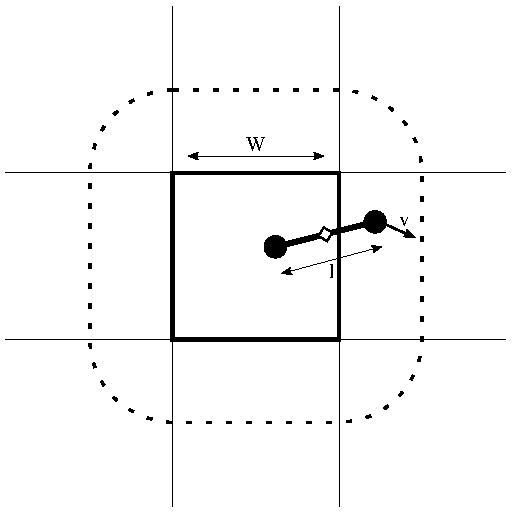
\includegraphics[height=0.3\textheight]{img/taille_boite}
	\caption{Éloignement maximal d'un segment.}
	\label{fig:taille-boite}
\end{figure}

Lorsque la largeur de la boite $W$ est supérieure au double de l'éloignement maximal, deux objets qui sont dans des boites non voisines ne peuvent pas entrer en collision. La largeur minimale de la boite pour vérifier cette condition est :

\begin{equation}
W_{min} = l_{max} + 2v_{max} + 2\epsilon
\end{equation}

La taille de la boite est alors légèrement agrandie pour que le domaine comporte un nombre entier de boites dans chaque dimension. 

\paragraph{Variantes}
D'autres solutions que le découpage en grille uniforme sont possibles. Certaines sont documentées dans \citecol{ericson2004real}, et notamment le découpage de l'espace en BSP-tree. Le découpage en grille uniforme à cependant été retenu car les géométries utilisées dans la dynamique des dislocations restent relativement homogènes et uniformes.


\subsubsection{Sphères englobantes}
\label{sec:spheres_englobantes}
Afin de réduire al complexité des primitives de test, il est possible d'utiliser des volumes englobants (\textit{bounding volumes}). Le principe consiste à inscrire les objets à tester pour la collision dans un volume, puis à tester l'intersection de ces volumes. Cette technique qui vise à rejeter certaines paires d'objets qui ne peuvent pas entrer en collision est appelée \textit{fast reject}. Les caractéristiques d'un fast-reject efficace sont les suivantes:
\begin{itemize}
	\item Pas de faux négatif : aucune collision ne doit être oubliée;
	\item Plus rapide que le test exact;
	\item Peu de faux négatif : les couples qui n'entrent pas en collision doivent être filtrés le mieux possible.
\end{itemize}

Les volumes utilisés sont des sphères. Chaque segment est simplifié par deux sphères centrées sur les quarts de segments de rayon $\frac{l}{4} + \epsilon$, comme l'illustre la figure \ref{fig:fastreject-segment}.

\begin{figure}[H]
	\centering
	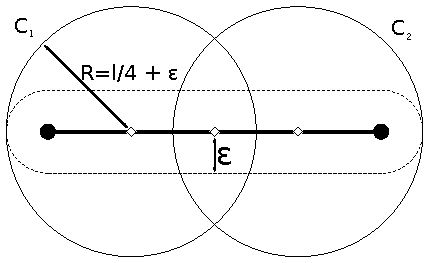
\includegraphics[width=0.7\textwidth]{img/fastreject-segment}
	\caption{Simplification d'un segment par deux sphères englobantes.}
	\label{fig:fastreject-segment}
\end{figure}

Lors de la détection de collisions, une première étape détecte la collision entre les sphères englobantes. Ensuite 
les points et les segments contenus dans les sphères qui entrent en collision sont testés. Les sphères $C_1$ et $C_2$ qui entrent en collision contiennent respectivement les points $n_1$ et $n_2$ ainsi que la moitié des segments $s_1$ et $s_2$. Les collisions exactes sont testées en utilisant les primitives de collision dans cet ordre :
\begin{itemize}
	\item Collision $n_1$ / $n_2$;
	\item Collisions $s_1$ / $n_2$ et $s_2$ / $n_1$;
	\item Collision $s_1$ / $s_2$.
\end{itemize}
La première collision exacte trouvée est ajoutée à la liste des collisions détectées. Les deux collisions point / segment peuvent être ajoutées en même temps si elles se produisent.

\paragraph{}
Le découpage en grille uniforme peut être utilisé pour la détection de collision entre sphères, et la taille de boite peut être raffinée. Le diamètre des sphères étant de l'ordre le la moitié de la longueur d'un segment, il est possible d'utiliser des boites plus petites, et donc de réduire la complexité du calcul. La largeur minimale d'une boite devient alors:

\begin{equation}
\begin{split}
W_{min} &= 2r_{max} + 2v_{max} \\
	    &= l_{max}/2 + 2v_{max} + 2\epsilon
\end{split}
\end{equation}



\subsubsection{Implémentation}

\paragraph{Structure de données}
Pour chaque segment, les sphères englobantes sont fabriquées. Le centre $\vect{c_i}$, la vitesse $\vect{v_i}$ et le rayon $r_i$ de chaque sphère sont calculés et stockés dans une structure données triée selon le découpage en grille uniforme. \`A chaque sphère sont aussi associés les indices du nœud $n_i$ et du segment $s_i$ qu'elle contient. Cette structure de données est comparable à un octree FMM ne contenant que des feuilles. La structure permet d'accéder à la liste des sphères contenues dans une boite de la grille.

La solution choisie pour implémenter ce conteneur consiste en un tableau $T$ trié par indice de morton indexé par une table de hachage $H$. Les sphères sont placées dans le tableau $T$ trié selon la z-curve (figure \ref{fig:z-curve}). La table de hachage est utilisée pour associer un intervalle $I_{ijk}$ du tableau $T$ à une case de la grille indexée par sa position ${i,j,k}$ ou son indice de Morton. Pour parcourir les sphères d'une boite ${i,j,k}$, il faut interroger la table de hachage pour obtenir l'intervalle $I_{ijk}$ du tableau à parcourir.\footnote{ Le tableau $T$ est en fait implémenté en Structure of Arrays au lieu de Array of Structures afin d'améliorer la performance.}	

\begin{figure}[H]
\begin{minted}[linenos=true,bgcolor=gray!10,mathescape,tabsize=2]{cpp} 
struct Sphere_Blocks{
	//Types
	struct Sphere{
		double center_x, center_y, center_z;//$c_i$ : Centre de la sphère 
		double v_x, v_y, v_z;               //$v_i$ : Vitesse de déplacement
		double r;                           //$r_i$ : Rayon de la sphère
		NodeIndex node;                     //$n_i$ : Noeud contenu dans la sphère
		SegmentIndex segment;               //$s_i$ : Segment contenu dans la sphère
	};	
	struct Indice_Block{                  //Position du bloc dans la grille
		int i,j,k;
	};
	struct Intervalle{                    //Intervalle dans le tableau T
		int min, max;
	}
	
	//Données
	std::vector< Sphere > T;               //Tableau contenant les sphères
	                                       //Table de hachage contenant les $I_{ijk}$
	std::unordered_map< Indice_Block, Intervalle > H;
};
\end{minted}
\caption{Structure de données contenant les sphères dans la grille uniforme.}
\label{fig:structure_grille}
\end{figure}



\paragraph{Parcours des objets}
L'algorithme se décompose en deux phases. La première phase (\textit{Broad Phase}) filtre les paires d'objets trop éloignées pour avoir une chance d'entrer en collision. La seconde phase (\textit{Narrow Phase}) s'occupe de détecter exactement les collisions, en extrayant des informations importantes pour la suite, à savoir la position et le temps où à lieu la collision. Les collisions probables détectées lors de la première phase sont enregistrées dans une liste temporaire pour être vérifiées lors de la seconde phase.

\begin{algorithm}[H]
	\SetAlgoLined
	\LinesNumbered
	\SetAlgoNoEnd	
	\DontPrintSemicolon
	\SetKwFunction{approxcol}{test\_collision\_spheres}
	\SetKwFunction{exactcol}{detect\_exact\_collisions}
	\SetKwFunction{Insert}{Insert}
	\KwData{Grille uniforme $\{H,T\}$ contenant les sphères. (Figure \ref{fig:structure_grille})}
	\KwResult{Liste des collisions $C$}
	$C_{preselected} \longleftarrow \{\}$\;
	\For{ $b_1$ bloc de la grille }
	{
		\For{ $b_2$ voisin de $b_1$ }
		{
			\For{ $i_1$ indice dans la boite $b_1$ }
			{
				\For{ $i_2$ indice dans la boite $b_2$ }
				{
					\If{ \approxcol{T[$i_1$], T[$i_2$]} }
					{
						$C_{preselected}$.\Insert{$\{i_1,i_2\}$}\;
					}
				}
			}
		}
	}
	$C \longleftarrow \{\}$\;
	\For{ $\{i_1,i_2\}$ dans $C_{preselected}$ }
	{
		$C_{spheres} \longleftarrow $ \exactcol{T[$i_1$], T[$i_2$]}\;
		$C$.\Insert{$C_{spheres}$}\;
	}

\caption{Détection de collisions}
\end{algorithm}

\begin{itemize}
	\item \texttt{test\_collision\_spheres} Utilise la primitive de collision de la section \ref{sec:detection-pointpoint} pour déterminer si les sphères entrent en collision;
	\item \texttt{detect\_exact\_collisions} détecte les collisions exactes entre les objets contenus dans les spheres, comme décrit en section \ref{sec:spheres_englobantes} et en retourne la liste.
\end{itemize}


\subsubsection{Parallélisation}
\label{sec:parallelisation_detection}
Qu'il s'agisse d'une parallélisation en mémoire partagée ou distribuée, l'algorithme de détection de collision se parallélise facilement. Chaque test de collision étant indépendant, il est possible de distribuer le travail sur plusieurs processeurs de calcul. 

\paragraph{Distribution du travail}
La méthode choisie consiste à distribuer les blocs de sphères lors de la \textit{Broad Phase}. A chaque processeur on assigne un ensemble de blocs à traiter que l'on appellera \textbf{blocs locaux}. L'algorithme se déroule de la même manière que précédemment à la différence que chaque processeur ne parcoure que ses blocs locaux. Chaque processeur enregistre une liste locale des collisions présélectionnées lors de la phase de collision entre sphères, pour ensuite effectuer la détection exacte de collision. Les collisions exactes sont stockées dans les listes locales aux threads qui doivent être fusionnées pour obtenir la liste globale des collisions.

\paragraph{Données distribuées}
Lorsque les données sont distribuées (MPI), les sphères sont distribuées de manière à ce que chaque processus en possède un nombre équivalent à traiter. Le load balancing des sphères utilise un algorithme inspiré de \citecol{cheng2005sort}, et permet d'obtenir un intervalle de blocs par processus. Les blocs d'un processus sont contigus selon la z-curve, ce qui permet de garder une cohérence spatiale. Les blocs à la frontière d'un domaine forment une zone de \textit{ghosts} qui doit être dupliquée sur plusieurs processus.

La distribution des segments et des sphères sur les différents processus peut ne pas correspondre à la distribution des sphères. Certains nœuds ou segments peuvent ne pas être locaux au moment du calcul des collisions exactes. Il faut donc communiquer les données des objets distants référencés dans la liste des collisions présélectionnées.

\end{document}
